%!TEX root = ../../PhD_thesis__Edouard_Leurent

\graphicspath{{2-Chapters/2-Chapter/}}

\chapter{Literature Review}
\label{chapter:2}

\begin{flushright}
	\begin{tabular}{@{}l@{}}
		\emph{Souhaite que la route soit longue. [\dots]}\\
		\emph{Visite aussi beaucoup de villes égyptiennes,}\\
		\emph{et n’aie de cesse de t’instruire auprès de ceux qui savent.}\\
	\end{tabular}
	
	Konstantinos Kavafis, \href{https://eleurent.github.io/sisyphe/texts/ithaki.html}{\emph{Ithaque}}.
\end{flushright}

\section{Sequential decision-making}
\label{sec:sequential-decision-making}

The skill of driving a car involves taking a series of decisions, where early stages influence the resulting outcomes and subsequent reasoning at late stages. This aspect is known as sequential (or multistage) decision-making. Let us start by introducing some useful notations. At each time step $t$, the system is described by its \emph{state} $s_t$ that belongs to a measurable state space $\cS$. Then, the agent can take an \emph{action} $a_t$ within a measurable action space $\cA$, before transitioning to a next state $s_{t+1}\in\cS$, drawn from a conditional distribution $P\parentheses{s_{t+1} \mid s_t, a_t}$ that we call the \emph{system dynamics}. The agent actions can themselves be drawn from a distribution $\pi\parentheses{a_t\mid s_t}$, called the \emph{policy}. This section describes the main design principles for coming up with a good driving policy $\pi$.

\subsection{Motion Planning}

The development of motion planning techniques for intelligent vehicles date back to the late 80s, supported by international research projects such as Eureka (1987) of the Prometheus program, followed by the DARPA Grand and Urban Challenges (2004, 2007), and more recently the VIAC (2010), GCDC (2011) and Delphi (2015) challenges. In two surveys \citep{Gonzalez2016,Paden2016} studying the literature of this period, three main approaches have been identified.

\paragraph{Search-based algorithms}

This method is based on a regular discrete partition of the state space $\cS$ called a \emph{lattice}, which must be connected by feasible state transitions \citep[\eg][]{Pivtoraiko2005}. This framing reduces motion planning to the problem of finding a shortest path in a known graph. Then, traditional graph-search algorithms such as Dijkstra's algorithm \citep{Dijkstra1959}, $A^\star$ \citep{Hart1968} or $D^\star$ \citep{Stentz1994} can been used to compute the optimal trajectory. This technique has been applied by at least five different teams during the DARPA Urban Challenge for driving on structured roads and unstructured parking: Dijkstra for team Ben Franklin \citep{Bohren2008} and VictorTango \citep{Bacha2008}, and $A^\star$ for Stanford University \citep{Montemerlo2008} and KIT \citep{Kammel2008}, and $D^\star$ by the winning team from CMU \citep{Urmson2008}.

\begin{figure}[tp]
	\centering
	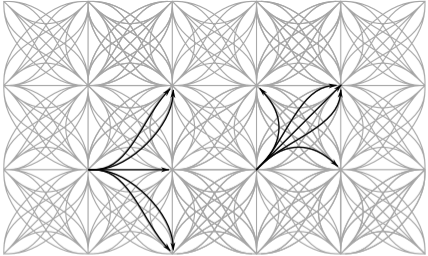
\includegraphics[width=0.5\linewidth]{img/lattice2}
	\caption{TODO: lattice}
\end{figure}

\paragraph{Sampling-based algorithms}

The limitation of search-based algorithms lies in the difficulty of formulating a regular lattice structure which feasible transitions between configurations, and in the real-time constraint that may not be met by graph-search algorithms. To address them, sampling-based motion planners iteratively grow a set of reachable configurations by randomly sampling valid transitions. The most popular ones are Probabilistic Roadmap (PRM) \citep{Kavraki1996}, Rapidly-exploring Random Trees (RRT) \citep{Lavalle98,Karaman2011} and Monte-Carlo Tree Search algorithms \citep[e.g.][]{Kocsis2006}.
\TODO{these methods are used in the context of AD in...}

\paragraph{Optimisation-based algorithms}

The third approach consists in directly optimizing a parametrized trajectory. An example is interpolation between the current and goal states, which has been applied to various classes of functions in the context of Autonomous Driving, such as lines and circles \citep{Reeds1990}, clothoids \citep{Funke2012}, polynomials \citep{Xu2012}, and Bézier curves \citep{Gonzalez}.

Motion planning techniques thus rely on deterministic models of the vehicle dynamics. These models are often required to take a simple form so that the search or optimisation procedure can be solved efficiently. Therefore, other objects are considered static and complex behaviours such as interactions between vehicles are left-out.
\TODO{collaborative planning, centralized (joint behaviour is optimised): does not allow human drivers, uncertainty. example ref: https://ieeexplore.ieee.org/document/736775}
Consequently, these techniques have mainly been successfully applied to the control of a single vehicle to track a sequence of known waypoints with static obstacles.

\subsection{Imitation Learning}

An orthogonal strategy to motion planning techniques is to learn a reactive policy $\pi(a|s)$ under supervision of an expert $\pi_E$ that produces a dataset $\cD$ of demonstration trajectories. To that end, a parametrized policy $\pi_\theta$ is optimised to minimise a regression loss $\cL$, for instance the $KL$ divergence to the expert actions distribution:
\begin{equation*}
\min_\theta \expectedvalue_{s\sim \cD} \left[\cL\left(\pi_{\theta}(a|s), \pi_E(a|s)\right)\right]
\end{equation*}

This approach is particularly suited when only low-level high-dimensional inputs are available, such as camera images, which prevents access to the dynamics model required by motion planning approaches. 
The first application of imitation learning to autonomous driving is the ALVINN (Autonomous Land Vehicle In a Neural Network) project \citep{Pomerleau89}, where a 3-layer neural network was trained for the task of road following, as shown in \Cref{fig:alvinn}.

\begin{figure}[tp]
	\centering
	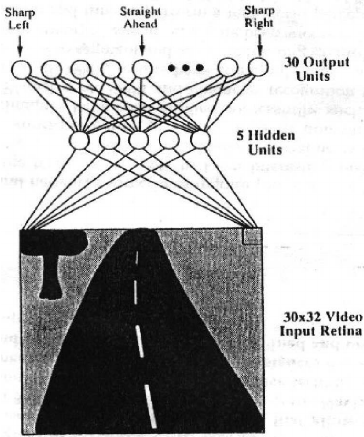
\includegraphics[width=0.4\linewidth]{img/alvinn}
	\caption{The 3-layer architecture used in ALVINN \citep{Pomerleau89}.}
	\label{fig:alvinn}
\end{figure}

\TODO{Compounding errors: \emph{"Supervised learning will not produce a policy with good long-horizon
performance, since a small mistake on the part of the policy will place the system
into states that are outside the distribution in the training data"} \citep{Levine2016}}
\TODO{ref needed: Dagger.}

\begin{figure}[tp]
	\centering
	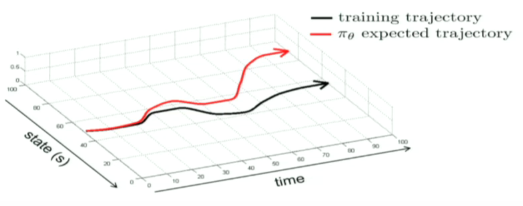
\includegraphics[width=0.7\linewidth]{img/cp4}
	\caption{TODO: Compounding errors}
\end{figure}

To mitigate this issue, \citep{Bojarski2016} proposed to simulate deviations from the expert trajectories using side cameras. The corresponding expert action labels were obtained by adding a constant steering wheel angle to adjust.

\citep{Eraqi2017,Xu2017} proposed to consider temporal dependencies by using recurrent neural networks.

\citep{Kuefler2017,Bhattacharyya2018} used Generative Adversarial Networks to...

But simply imitating is not enough, we need to control the agent / condition the policy with a goal. \citep{Codevilla2018}

\subsection{Reinforcement Learning}

Reinforcement Learning is a general decision-making framework formulated as an optimal control problem. It is typically formalized as a \emph{Markov Decision Process} (MDP), in which at each time step $t$, an agent observes its current state $s_t\in S$ and picks an action $a_t\in A$, before transitioning to a next state $s_{t+1}\in S$ drawn from a transition distribution $P(s_{t+1}|s_t,a_t)$ and receiving a bounded reward $r_t\in[0, 1]$ drawn from a reward distribution $P(r_t|s_t,a_t)$. The agent must act so as to optimise in expectation its cumulative discounted reward, also called \emph{return}, where $\gamma\in[0,1)$ is the discount factor:

\begin{equation*}
\max_{\pi}\expectedvalue_{\pi, P} \left[\sum_t \gamma^t r_t\right].
\end{equation*}

Convenient framework for analysis, but it's often too narrow a frame for the real world to fit in. In the following, we will enumerate several assumptions behind the MDP framework that may not hold in practice, and for which variants have been developed. We will focus on applications of the variants the particular context of Autonomous Driving.

\section{States and partial observability}

The first modelling assumption of the MDP framework is that the agent perfectly knows its own state $s\in\cS$. In practice, information about the scene can only be obtained through sensors, which produce typically noisy measurements. In addition to noise, some part of the state may simply be missing: occlusion.
\TODO{Insert image of partial observability}

Proposed model: POMDP.
Belief state propagation: Kalman filtering for linear system and gaussian noise.
Algo: PBVI, POMCP

Examples:
- Sensor noise: [Probabilistic Online POMDP Decision Making for Lane Changes in Fully Automated Driving]
- Motion planning for a UAV with no GPS, landmark localization: [A POMDP Approach to Robot Motion Planning under Uncertainty]. 
- Planning at an intersection with a moving occluded obstacle (8D system): [Solving Continuous POMDPs:  Value Iteration with Incremental Learning of an Efficient Space Representation]
- ?? : [Probabilistic decision-making under uncertainty for autonomous driving using continuous POMDPs]
- The other drivers locations are observed but not their intentions [Intention-Aware Motion Planning]. MOMDP framework.
- [ Probabilistic Decision-Making at Road Intersections: Formulation and Quantitative Evaluation ]
- Kalman + POMCP for intersection [https://arxiv.org/abs/1704.04322]
- Sunberg: evaluate the POMDP vs MDP approximation with an assumed internal state.
 

\section{Actions and temporal abstraction}
\section{Rewards and inverse reinforcement learning}
\section{Dynamics and transfer}
\section{Optimisation criterion and safety}
